\input{../utils/preamble}
\createdgmtitle{4}
%--------------------------------------------------------------------------------
\begin{document}
%--------------------------------------------------------------------------------
\begin{frame}
%\thispagestyle{empty}
\titlepage
\end{frame}
%=======
\begin{frame}{Bayesian framework}
	\begin{block}{Bayes theorem}
		\[
			p(\bt | \bx) = \frac{p(\bx | \bt) p(\bt)}{p(\bx)} = \frac{p(\bx | \bt) p(\bt)}{\int p(\bx | \bt) p(\bt) d \bt} 
		\]
		\begin{itemize}
			\item $\bx$ -- observed variables, $\bt$ -- unobserved variables (latent variables/parameters);
			\item $p(\bx | \bt)$ -- likelihood;
			\item $p(\bx) = \int p(\bx | \bt) p(\bt) d \bt$ -- evidence;
			\item $p(\bt)$ -- prior distribution, $p(\bt | \bx)$ -- posterior distribution.
		\end{itemize}
	\end{block}
	\begin{block}{Meaning}
		We have unobserved variables $\bt$ and some prior knowledge about them $p(\bt)$. Then, the data $\bx$ has been observed. 
		Posterior distribution $p(\bt | \bx)$ summarizes the knoweldge after the obbservations.
	\end{block}
\end{frame}
%=======
\begin{frame}{Variational Lower Bound}
    We are given the set of objects $\bX = \{\bx_i\}_{i=1}^n$. 
    The goal is to perform bayesian inference on the unobserved variables $\bT = \{\bt_i\}_{i=1}^n$.
    \begin{block}{Evidence Lower Bound (ELBO)}
    \vspace{-0.3cm}
        \begin{multline*}
    		\log p(\bX) 
    		= \log \frac{p(\bX, \bT)}{p(\bT|\bX)} = \\ 
    		= \int q(\bT) \log \frac{p(\bX, \bT)}{p(\bT|\bX)}d\bT
    		= \int q(\bT) \log \frac{p(\bX, \bT) q(\bT)}{p(\bT|\bX) q(\bT)} d\bT = \\
    		= \int q(\bT) \log \frac{p(\bX, \bT)}{q(\bT)}d\bT + \int q(\bT) \log \frac{q(\bT)}{p(\bT|\bX)}d\bT = \\ 
    		= \mathcal{L} (q) + KL(q(\bT) || p(\bT|\bX)) \geq \mathcal{L} (q).
    	\end{multline*}
        \vspace{-0.3cm}
    \end{block}
	We would like to maximize lower bound $\mathcal{L}(q)$.
\end{frame}
%=======
\begin{frame}{Mean field approximation}
    \begin{block}{Independence assumption}
    \vspace{-0.3cm}
    \[
    q(\bT) = \prod_{i=1}^k q_i(\bT_i), \quad \bT = [\bT_1, \dots, \bT_k], \, \bT_j = \{ \bt_{ij}\}_{i=1}^n, \, \bt_i = \{ \bT_{ij}\}_{j=1}^k.
    \]
    \vspace{-0.3cm}
    \end{block}
    \begin{block}{Block coordinate optimization of ELBO for $q_j(\bT_j)$}
  
    {\footnotesize
    \vspace{-0.3cm}
        \begin{multline*}
    		\mathcal{L} (q)
    		= \int q(\bT) \log \frac{p(\bX, \bT)}{q(\bT)}d\bT
    		= \int \left[\prod_{i=1}^k q_i(\bT_i) \right] \log \frac{p(\bX, \bT)}{\left[\prod_{i=1}^k q_i(\bT_i) \right]}  \prod_{i=1}^k d \bT_i = \\
    		= \int \left[ \prod_{i=1}^k q_i \right] \log p(\bX, \bT) \prod_{i=1}^k d \bT_i  
    		- \sum_{i=1}^k \int \left[ \prod_{j=1}^k q_j \right] \log q_i \prod_{j=1}^k d \bT_j = \\
    		= \int q_j \left[\int  \log p(\bX, \bT) \prod_{i \neq j} q_i d \bT_i \right] d \bT_j - \\
    		- \int q_j \log q_j d\bT_j + \text{const}(q_j) \rightarrow \max_{q_j}
    	\end{multline*}
        \vspace{-0.3cm}}
    \end{block}
\end{frame}
%=======
\begin{frame}{Mean field approximation}
	\footnotesize
	\begin{block}{Block coordinate optimization of ELBO for $q_j(\bT_j)$}
		\vspace{-0.4cm}
	    \begin{multline*}
			\mathcal{L} (q) 
			= \int q_j \left[\int \log p(\bX, \bT) \prod_{i \neq j} q_i d \bT_i \right] d \bT_j
			- \int q_j \log q_j  d\bT_j + \text{const}(q_j) = \\
			= \int q_j \log \hat{p}(\bX, \bT_j) d \bT_j 
			- \int q_j \log q_j d\bT_j + \text{const}(q_j) \rightarrow \max_{q_j}.
		\end{multline*}
		Here we introduce
		\[
		   \log \hat{p}(\bX, \bT_j) = \int \log p(\bX, \bT) \prod_{i \neq j} q_i d \bT_i = \mathbb{E}_{i \neq j} \log p(\bX, \bT) + \text{const}(q_j)
		\]
	    \end{block}
	    \vspace{-0.3cm}
	    \begin{block}{Final ELBO derivation for $q_j(\bT_j)$}
	    	\vspace{-0.5cm}
			\begin{multline*}
	    		\mathcal{L} (q)
	    		= \int q_j (\bT_j) \log \hat{p}(\bX, \bT_j) d \bT_j - \int q_j(\bT_j) \log q_j(\bT_j) d\bT_j + \text{const}(q_j) = \\
	    		 \int q_j (\bT_j) \log \frac{\hat{p}(\bX, \bT_j)}{q_j(\bT_j)} d\bT_j + \text{const}(q_j) = \\
	    		= - KL (q_j(\bT_j) || \hat{p}(\bX, \bT_j)) + \text{const}(q_j) \rightarrow \max_{q_j}.
	    	\end{multline*}
	    \end{block}
\end{frame}
%=======    
\begin{frame}{Mean field approximation}   
	 \begin{block}{Independence assumption}
		\vspace{-0.3cm}
		\[
		q(\bT) = \prod_{i=1}^k q_i(\bT_i), \quad \bT = [\bT_1, \dots, \bT_k], \quad \bT_j = \{ \bt_{ij}\}_{i=1}^n.
		\]
		\vspace{-0.3cm}
	\end{block}
	\begin{block}{ELBO}
	    \[
			\mathcal{L} (q) = - KL (q_j(\bT_j) || \hat{p}(\bX, \bT_j))  + \text{const}(q_j) \rightarrow \max_{q_j}.
	    \]
	    \vspace{-0.3cm}
	\end{block}
	 \begin{block}{Solution}
	 	\vspace{-0.3cm}
		 \[
		    q_j(\bT_j) = \text{const} \cdot \hat{p}(\bX, \bT_j)
		 \]
		 \[
		 	\log \hat{p}(\bX, \bT_j) = \mathbb{E}_{i \neq j} \log p(\bX, \bT) + \text{const}
		 \]
		 \[
		     \log q_j(\bT_j) = \mathbb{E}_{i \neq j} \log p(\bX, \bT) + \text{const}
		 \]
		 \vspace{-0.3cm}
	 \end{block}
\end{frame}
%=======
\begin{frame}{Mean field approximation}
	\begin{block}{ELBO}
		\[
			\mathcal{L} (q) = - KL (q_j(\bT_j) || \hat{p}(\bX, \bT_j))  + \text{const}(q_j) \rightarrow \max_{q_j}.
		\]
		\vspace{-0.3cm}
	\end{block}
	\begin{block}{Solution}
		\vspace{-0.3cm}
		\[
			\log q_j(\bT_j) = \mathbb{E}_{i \neq j} \log p(\bX, \bT) + \text{const}
		\]
		\vspace{-0.3cm}
	\end{block}
	Let assume 
	\begin{itemize}
		\item $\bT = [\bT_1, \bT_2] = [\bZ, \btheta]$, $q(\bT) = q(\bT_1) \cdot q(\bT_2) = q(\bZ) \cdot q(\btheta)$.
		\item restrict the class of probability distribution for $\btheta$ to Dirac delta functions:
		\[
			q_2 = q(\bT_2) = q(\btheta) = \delta(\btheta - \btheta^*).
		\]
		
		Under the restrictions the exact solution for $q_2$ is not reached (KL could be greater than 0).
	\end{itemize}
\end{frame}
%=======
\begin{frame}{Mean field approximation}
	\begin{block}{General solution}
		\vspace{-0.3cm}
		\[
		\log q_j(\bT_j) = \mathbb{E}_{i \neq j} \log p(\bX, \bT) + \text{const}
		\]
		\vspace{-0.3cm}
	\end{block}
	\begin{block}{Solution for $q_1 = q(\bZ)$}
		\vspace{-0.3cm}
		\begin{multline*}
			\log q(\bZ) = \int q(\btheta) \log p(\bX, \bZ,  \btheta) d\btheta + \text{const} = \\
			= \int \delta(\btheta - \btheta^*) \log p(\bX, \bZ,  \btheta) d\btheta + \text{const} = \\
			= \log p (\bZ | \bX, \btheta^*) +  \text{const}.
		\end{multline*}
	\end{block}
	\vspace{-0.3cm}
	\begin{block}{EM-algorithm (E-step)}
		\vspace{-0.3cm}
	\[
		q(\bZ) = \argmax_q \mathcal{L} (q, \btheta^*) = \argmin_q KL(q || p) = p(\bZ| \bX, \btheta^*).
	\]
	\end{block}
\end{frame}
%=======
\begin{frame}{Mean field approximation}
	\begin{block}{ELBO}
		\[
			\mathcal{L} (q) = - KL (q_j(\bT_j) || \hat{p}(\bX, \bT_j))  + \text{const}(q_j) \rightarrow \max_{q_j}.
		\]
	\vspace{-0.3cm}
	\end{block}
	\begin{block}{ELBO maximization w.r.t. $q_2 = q(\btheta) = \delta(\btheta - \btheta^*)$}
		\vspace{-0.3cm}
		\begin{align*}
			\mathcal{L} (q_1, q_2) &= - KL (q(\btheta) || \hat{p}(\bX, \btheta))  + \text{const}(\btheta^*) \\ 
			&= \int q (\btheta) \log \frac{\hat{p}(\bX, \btheta)}{q(\btheta)} d\btheta + \text{const}(\btheta^*) \\
			& = \int q (\btheta) \log \hat{p}(\bX, \btheta) d\btheta  - \int q (\btheta) \log q(\btheta) d\btheta + \text{const}(\btheta^*) \\
			& = \int \delta(\btheta - \btheta^*) \log \hat{p}(\bX, \btheta) d\btheta + \text{const}(\btheta^*) \rightarrow \max_{\btheta^*}
		\end{align*}
		\vspace{-0.3cm}
	\end{block}
\end{frame}
%=======
\begin{frame}{Mean field approximation}
	
	\begin{block}{ELBO maximization w.r.t. $q_2 = q(\btheta) = \delta(\btheta - \btheta^*)$}
		\vspace{-0.3cm}
		\begin{multline*}
			\mathcal{L} (q_1, q_2) = \int \delta(\btheta - \btheta^*) \log \hat{p}(\bX, \btheta) d\btheta + \text{const}
			= \log \hat{p}(\bX, \btheta^*)  + \text{const} \\
			= \mathbb{E}_{i \neq j} \log p(\bX, \bT) + \text{const} = \mathbb{E}_{q_1} \log p(\bX, \bZ, \btheta^*) + \text{const} \\
		= \int q(\bZ) \log p(\bX, \bZ|  \btheta^*) d\bZ + \log p(\btheta^*)+ \text{const}\rightarrow \max_{\btheta^*}
	\end{multline*}
	\end{block}
	\vspace{-0.3cm}
	\begin{block}{EM-algorithm (M-step)}
		\vspace{-0.3cm}
		 \begin{align*}
		 	\mathcal{L}(q, \btheta) &= \int q(\bZ) \log \frac{p(\bX, \bZ | \btheta)}{q(\bZ)}d\bZ \\
		 	&= \int q(\bZ) \log p(\bX, \bZ | \btheta) d\bZ + \text{const} \rightarrow \max_{\btheta}
		 \end{align*}
	\end{block}
\end{frame}
%=======
\begin{frame}{Mean field approximation}
    \begin{block}{Solution}
    \[
        \log q_j(\bT_j) = \mathbb{E}_{i \neq j} \log p(\bX, \bT) + \text{const}
    \]
    \end{block}

	\begin{block}{EM algorithm (special case)}
	\begin{itemize}
		\item Initialize $\btheta^*$;
		\item E-step
		\[
			q(\bZ) = \argmax_q \mathcal{L} (q, \btheta^*) = \argmin_q KL(q || p) =
			 p(\bZ| \bX, \btheta^*);
		\]
		\item M-step
		\[
			\btheta^* = \argmax_{\btheta} \mathcal{L} (q, \btheta);
		\]
		\item Repeat E-step and M-step until convergence.
	\end{itemize}
	\end{block}
\end{frame}
%=======
\begin{frame}{Likelihood-based models so far...}
	\begin{minipage}[t]{0.5\columnwidth}
		\begin{block}{Autoregressive models}
			\vspace{-0.5cm}
			\[
			p(\bx|\btheta) = \prod_{i=1}^m p(x_i | \bx_{1:i - 1}, \btheta)
			\]
			\vspace{-0.2cm}
			\begin{itemize}
				\item tractable likelihood, 
				\item no inferred latent factors.
			\end{itemize}
		\end{block}
	\end{minipage}%
	\begin{minipage}[t]{0.5\columnwidth}
		\begin{block}{Latent variable models}
			\[
			p(\bx| \btheta) = \int p(\bx, \bz | \btheta) d \bz
			\]
			\begin{itemize}
				\item latent feature representation, 
				\item intractable likelihood.
			\end{itemize}
		\end{block}
	\end{minipage}
	
	\vspace{1cm } 
	How to build model with latent variables and tractable likelihood?
\end{frame}
%=======
\begin{frame}{Flows intuition}
	Let $\xi$ be a random variable with density $p(\xi)$. Then
	\[
	\eta = F(\xi) = P(\xi < x) = \int_{-\infty}^\xi p(t)dt \sim U[0, 1].
	\]
	\[
		P(\eta < y) = P(F(\xi) < y) = P(\xi < F^{-1}(y)) = F(F^{-1}(y)) = y
	\]
	Hence
	\[
	\eta \sim U[0, 1]; \quad \xi = F^{-1}(\eta) \quad \xi \sim p(\xi).
	\]
	\begin{figure}
		\includegraphics[width=\linewidth]{figs/flows_1d}
	\end{figure}
	\myfootnotewithlink{https://sites.google.com/view/berkeley-cs294-158-sp19/home}{image credit: https://sites.google.com/view/berkeley-cs294-158-sp19/home}
	
\end{frame}
%=======
\begin{frame}{Flows intuition}
	\begin{itemize}
		\item Let $\bz \sim p(\bz)$ is a random variable with base distribution $p(\bz) = U[0, 1]^m$. 
		\item Let $\bx \sim p(\bx)$ is a random variable with complex distribution $p(\bx)$ and cdf $F(\bx)$. 
		\item Then noise variable $\bz$ could be transformed to $\bx$ using inverse cdf~$F^{-1}$ ($\bx = F^{-1}(\bz)$).
	\end{itemize}
	How to transform random variable $\bz$  which have distribution different from uniform to $\bx$?
		\begin{itemize}
			\item Let $\bz \sim p(\bz)$ is a random variable with base distribution $p(\bz)$ and cdf $G(\bz)$.
			\item Then $\bz_0 = G(\bz)$ has base distribution $p(\bz_0) = U[0, 1]^m$.
			\item Let $\bx \sim p(\bx)$ is a random variable with complex distribution $p(\bx)$ and cdf $F(\bx)$. 
			\item Then noise variable $\bz$ could be transformed to $\bx$ using cdf $G$ and inverse cdf~$F^{-1}$ ($\bx = F^{-1}(\bz_0) = F^{-1}(G(\bz))$).
		\end{itemize}
\end{frame}
%=======
\begin{frame}{Change of variables}
	\begin{block}{Theorem}
		Let 
		\begin{itemize}
			\item $\bx$ is a random variable with density function $p(\bx)$;
			\item $f: \mathbb{R}^m \rightarrow \mathbb{R}^m$ is a differentiable, invertible function (diffeomorphism);
			\item $\bz = f(\bx)$, $\bx = f^{-1}(\bz) = g(\bz)$ (here $g = f^{-1}$).
		\end{itemize}
		Then
		\[
		p(\bx) = p(\bz) \left|\det \left(  \frac{\partial \bz}{\partial \bx} \right) \right| = p(f(\bx)) \left|\det \left(  \frac{\partial f(\bx)}{\partial \bx} \right) \right|.
		\]
	\end{block}
	\begin{block}{Note}
		\begin{itemize}
			\item $\bx$ and $\bz$ have the same dimensionality (lies in $\bbR^m$);
			\item $ \left|\det \left(  \frac{\partial f(\bx)}{\partial \bx} \right)\right| = \left|\det \left(  \frac{\partial g^{-1}(\bx)}{\partial \bx} \right)\right| = \left|\det \left(  \frac{\partial g(\bz)}{\partial \bz} \right)\right|^{-1}$;
			\item $f(\bx, \btheta)$ could be parametric function.
		\end{itemize}
	\end{block}
\end{frame}
%=======
\begin{frame}{Fitting flows}
	\begin{block}{MLE problem}
		\vspace{-0.3cm}
		\[
		\btheta^* = \argmax_{\btheta} p(\bX | \btheta) = \argmax_{\btheta} \prod_{i=1}^n p(\bx_i | \btheta) = \argmax_{\btheta} \sum_{i=1}^n \log p(\bx_i | \btheta).
		\]
		\vspace{-0.3cm}
	\end{block}
	\begin{block}{Challenge}
		$p(\bx | \btheta)$ could be intractable.
	\end{block}
	\begin{block}{Fitting flow to solve MLE}
		\[
		p(\bx|\btheta) = p(\bz) \left|\det \left(  \frac{\partial \bz}{\partial \bx} \right) \right|  = p(f(\bx, \btheta)) \left|\det \left( \frac{\partial f(\bx, \btheta)}{\partial \bx} \right) \right|
		\]
		\[
			\log p(\bx|\btheta) = \log p(f(\bx, \btheta)) + \log  \left|\det \left( \frac{\partial f(\bx, \btheta)}{\partial \bx} \right) \right|
		\]
	\end{block}
\end{frame}
%=======
\begin{frame}{Flows}
	\begin{figure}
		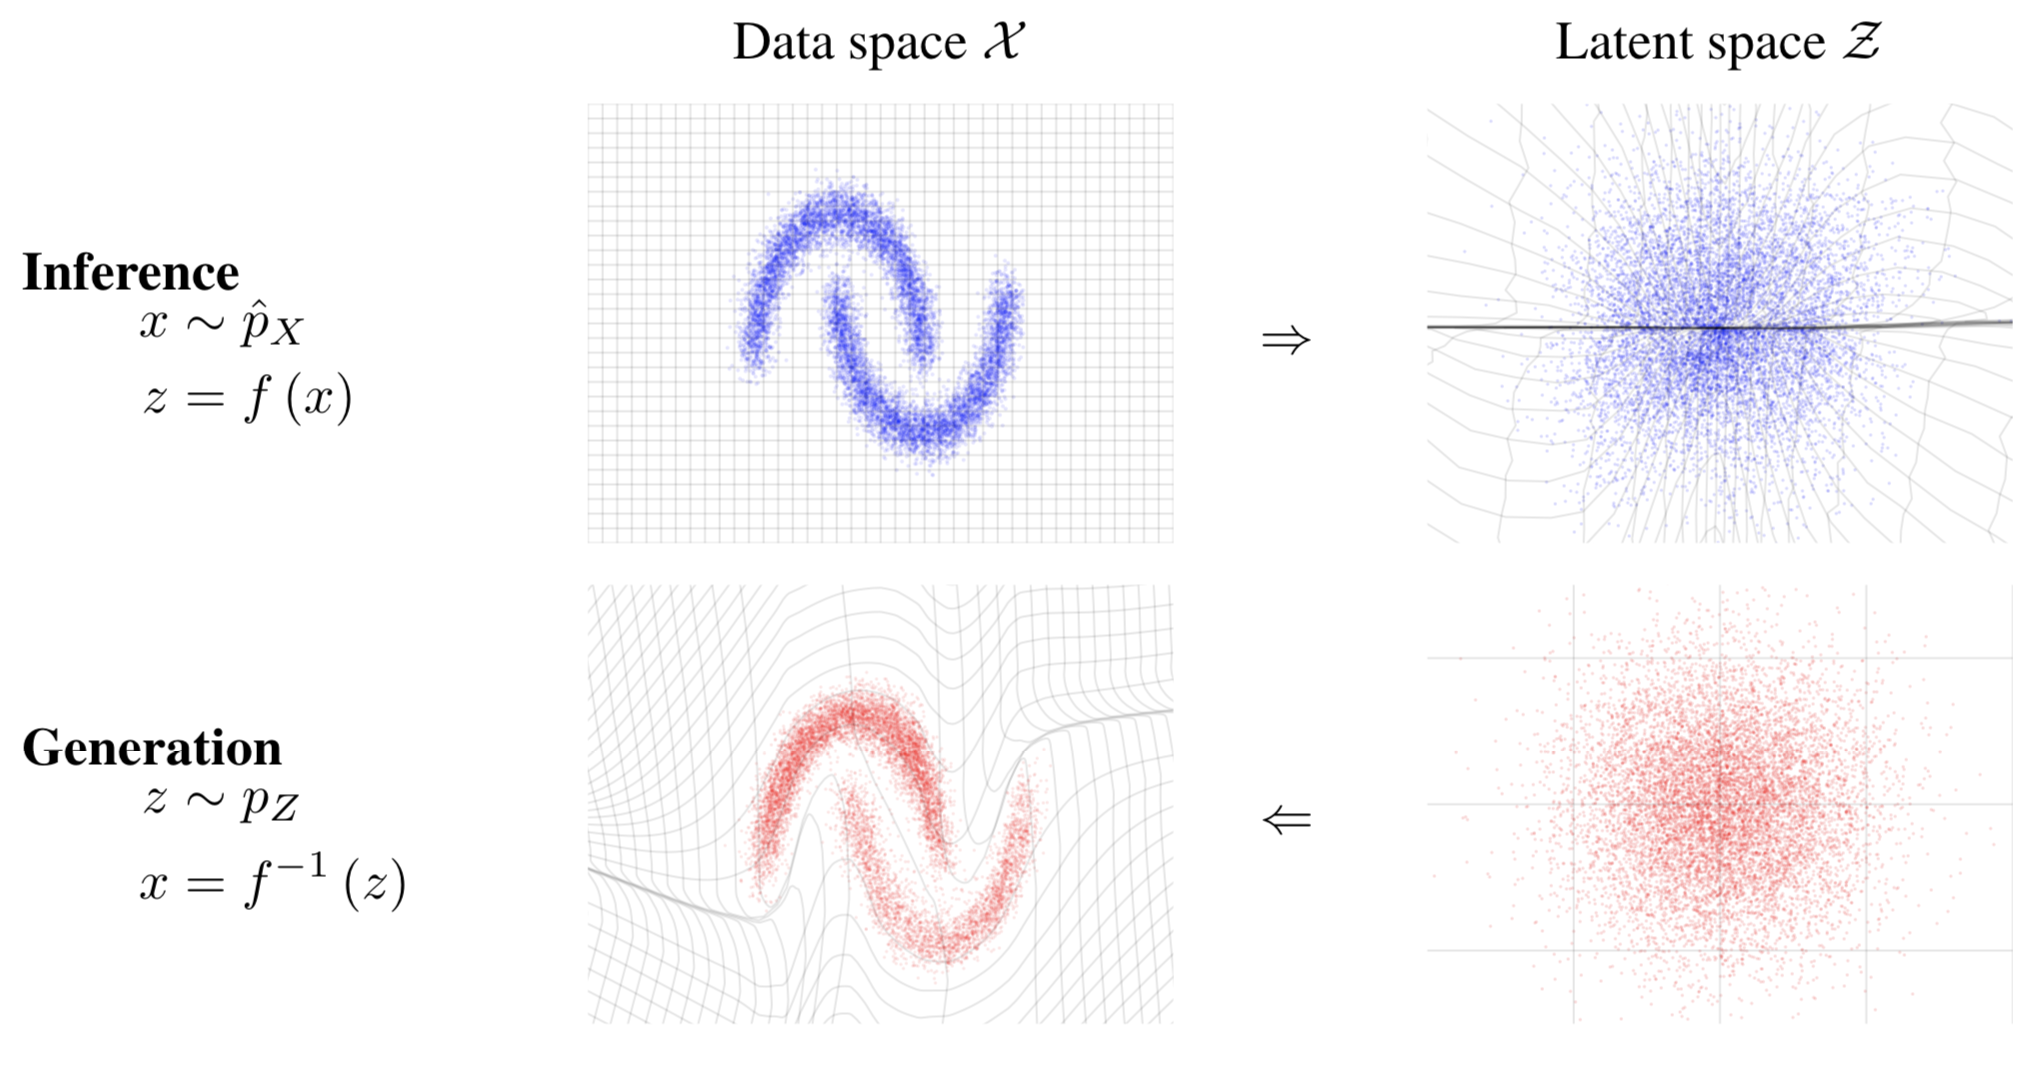
\includegraphics[width=0.7\linewidth]{figs/flows_how2.png}
	\end{figure}
	\vspace{-0.3cm}
	\begin{block}{Computational requirement}
		\begin{itemize}	
			\item Evaluating model density $p(\bx | \btheta)$, we  requires computing the transformation $\bz = f(\bx,  \btheta)$ and its Jacobian determinant $\left|\det \left( \frac{\partial f(\bx, \btheta)}{\partial \bx} \right) \right|$,
			and evaluating the density $p(\bz)$.
			\item Sampling $\bx$ from the model requires the ability to sample from $p(\bz)$ and to compute the transformation $\bx = g(\bz, \btheta) = f^{-1}(\bz, \btheta)$. 
		\end{itemize}
	\end{block}
	\myfootnotewithlink{https://arxiv.org/abs/1605.08803}{Dinh L., Sohl-Dickstein J., Bengio S. Density estimation using Real NVP, 2016} 
\end{frame}
%=======
\begin{frame}{Composition of flows}
	\begin{block}{Theorem}
		Diffeomorphisms are \textbf{composable} (If Let $f_1, f_2$ satisfy conditions of the change of variable theorem (differentiable and invertible), then $\bz = f(\bx) = f_2 \circ f_1(\bx)$ also satisfy it).
	\end{block}
	\begin{multline*}
		p(\bx) = p(\bz) \left|\det \left(  \frac{\partial \bz}{\partial \bx} \right) \right| = p(f(\bx)) \left|\det \left(  \frac{\partial f(\bx)}{\partial \bx} \right) \right| = \\
		= p(f(\bx)) \left|\det \left(\frac{\partial f_2 \circ f_1(\bx)}{\partial \bx} \right) \right| =
		p(f(\bx)) \left|\det \left(\frac{\partial \textbf{f}_2}{\partial \textbf{f}_1} \cdot \frac{\partial \textbf{f}_1}{\partial \bx} \right) \right| = \\
		= p(f(\bx))  \left|\det \left(\frac{\partial \textbf{f}_2}{\partial \textbf{f}_1} \right) \right| \cdot \left| \det \left( \frac{\partial \textbf{f}_1}{\partial \bx} \right) \right|
	\end{multline*}

	What will we get in the case $\bz = f(\bx) = f_n \circ \dots \circ f_1(\bx)$?
\end{frame}
%=======
\begin{frame}{Flows}
	\vspace{-0.3cm}
	\[
		\log p(\bx|\btheta) = \log p(f(\bx, \btheta)) + \log \left|\det \left( \frac{\partial f(\bx, \btheta)}{\partial \bx} \right) \right|
	\]
	\vspace{-0.3cm}
	\begin{block}{Definition}
		Normalizing flow is a \textit{differentiable, invertible} mapping from data $\bx$ to the noise $\bz$. 
	\end{block}
	\begin{itemize}
		\item "Normalizing" means that the inverse flow takes samples from $p(\bx)$ and normalizes them into samples from density $p(\bz)$.
		\item "Flow" refers to the trajectory that samples from $p(\bz)$ follow as they are transformed by the sequence of transformations
		\[
		\bz = f_K \circ \dots \circ f_1(\bx); \quad \bx = f_1^{-1} \circ \dots \circ f_K^{-1} (\bz) = g_1 \circ \dots \circ g_K(\bz) 
		\] 
		\begin{multline*}
			p(\bx) = p(f_K \circ \dots \circ f_1(\bx)) \left|\det \left(\frac{\partial f_K \circ \dots \circ f_1(\bx)}{\partial \bx} \right) \right| = \\
			= p(f_K \circ \dots \circ f_1(\bx)) \prod_{k=1}^K \left|\det \left(\frac{\partial \mathbf{f}_k}{\partial \mathbf{f}_{k-1}} \right) \right|.
		\end{multline*}
	\end{itemize}
\end{frame}
%=======
\begin{frame}{Flows}
	\[
	\log p(\bx|\btheta) = \log p(f(\bx, \btheta)) + \log \left|\det \left( \frac{\partial f(\bx, \btheta)}{\partial \bx} \right) \right|
	\]
	What is the complexity of the determinant computation?
	\begin{block}{What we want}
		\begin{itemize}
			\item Efficient computation of Jacobian $\frac{\partial f(\bx, \btheta)}{\partial \bx}$;
			\item Efficient sampling from the base distribution $p(\bz)$;
			\item Efficient inversion of $f(\bx, \btheta)$.
		\end{itemize}
		
	\end{block}
	
\end{frame}
%=======
\begin{frame}{Planar Flows}
	\vspace{-0.2cm}
	\[
	g(\bz, \btheta) = \bz + \mathbf{u} \, h(\bw^T\bz + b).
	\]
	\vspace{-0.2cm}
	\begin{itemize}
		\item $\btheta = \{\bu, \bw, b\}$;
		\item $h$ is a smooth element-wise non-linearity.
	\end{itemize}
	\begin{align*}
		\left| \det \left( \frac{\partial g(\bz, \btheta)}{\partial \bz} \right)\right| &= \left| \det \left( \bI +  h'(\bw^T \bz + b) \bw\bu^T\right) \right| \\
		&= \left| 1 + h'(\bw^T \bz + b) \bw^T \bu \right|
	\end{align*}
	The transformation is invertible if (just one of example)
	\[
	h = \tanh; \quad h'(\bw^T \bz + b) \bu^T \bw \geq -1.
	\]
	\myfootnotewithlink{https://arxiv.org/abs/1505.05770}{Rezende D. J., Mohamed S. Variational Inference with Normalizing Flows, 2015} 
\end{frame}
%=======
\begin{frame}{Planar Flows}
	\[
	\bz_K = g_1 \circ \dots \circ g_K (\bz); \quad g_k = g(\bz_k, \btheta_k).
	\]
	\begin{figure}
		\centering
		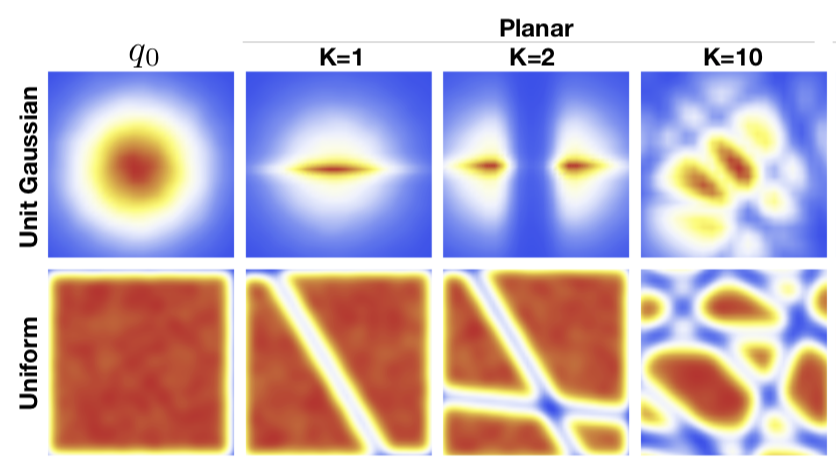
\includegraphics[width=0.9\linewidth]{figs/planar_flows.png}
	\end{figure}
	\myfootnotewithlink{https://arxiv.org/abs/1505.05770}{Rezende D. J., Mohamed S. Variational Inference with Normalizing Flows, 2015} 
\end{frame}
%=======
\begin{frame}{Jacobian structure}
	\begin{itemize}
		\item What is a determinant of a diagonal matrix?
		\[
		\bz = f(\bx, \btheta) = (f_1(x_1, \btheta), \dots, f_m(x_m, \btheta)).
		\]
		\[
		\log \left|\det \left( \frac{\partial f(\bx, \btheta)}{\partial \bx} \right) \right| = \log \left| \prod_{i=1}^m f_i'(x_i, \btheta) \right| = \sum_{i=1}^m \log \left| f_i'(x_i, \btheta) \right|.
		\]
		\item What is a determinant of a triangular matrix? \\
		Let $z_i$ depends only on $\bx_{1:i}$ (or without loss of generality $x_i$ depends on $\bz_{1:i}$). \\
		What is the inverse of such a transformation?
	\end{itemize}
\end{frame}
%=======
\begin{frame}{NICE}
	\begin{block}{Coupling layer}
		\begin{equation*}
			\begin{cases} \bz_{1:d} = \bx_{1:d} \\ \bz_{d:m} = \tau (\bx_{d:m}, c(\bx_{1:d}))\end{cases} \quad 
			\begin{cases} \bx_{1:d} = \bz_{1:d} \\ \bx_{d:m} = \tau^{-1} (\bz_{d:m}, c(\bz_{1:d}))\end{cases}
		\end{equation*}
		\begin{itemize}
			\item $c: \mathbb{R}^d \rightarrow \mathbb{R}^{k}$ -- coupling function;
			\item $\tau : \mathbb{R}^{m - d} \times c(\mathbb{R}^d) \rightarrow \mathbb{R}^{m - d}$ -- coupling law.
			\item 
			\[
			\det \left( \frac{\partial \bz}{\partial \bx} \right) = \det 
			\begin{pmatrix}
				\bI_d & 0_{d \times m - d} \\
				\frac{\partial \bz_{d:m}}{\partial \bx_{1:d}} & \frac{\partial \bz_{d:m}}{\partial \bx_{d:m}}
			\end{pmatrix} = 
			\det \left( \frac{\partial \bz_{d:m}}{\partial \bx_{d:m}} \right)
			\]
		\end{itemize}
	\end{block}
	\myfootnotewithlink{https://arxiv.org/abs/1410.8516}{Dinh L., Krueger D., Bengio Y. NICE: Non-linear Independent Components Estimation, 2014}
\end{frame}
%=======
\begin{frame}{NICE}
	\begin{block}{Coupling layer}
		\vspace{-0.8cm}
		\begin{equation*}
			\begin{cases} \bz_{1:d} = \bx_{1:d}; \\ \bz_{d:m} = \tau (\bx_{d:m}, c(\bx_{1:d}));\end{cases} 
			\quad \Rightarrow \quad 
			\begin{cases} \bx_{1:d} = \bz_{1:d}; \\ \bx_{d:m} = \tau^{-1} (\bz_{d:m}, c(\bz_{1:d})).\end{cases}
		\end{equation*}
		\vspace{-0.5cm}
	\end{block}
	\begin{block}{Coupling function $c(\cdot)$}
		Any complex function (without restrictions). For example, neural network.
	\end{block}
	\begin{block}{Coupling law $\tau(\cdot, \cdot)$}
		\begin{itemize}
			\item $\tau(x, c) = x + c$ -- \textit{additive};
			\item $\tau(x, c) = x \odot c, \, c \neq 0$ -- multiplicative;
			\item $\tau(x, c) = x \odot c_1 + c_2, \, c_1 \neq 0$ -- affine.
		\end{itemize}
	\end{block}
	To obtain more flexible class of dictributions, stack more coupling layers (with different ordering of components!). \\
	
	\myfootnotewithlink{https://arxiv.org/abs/1410.8516}{Dinh L., Krueger D., Bengio Y. NICE: Non-linear Independent Components Estimation, 2014}
\end{frame}
%=======
\begin{frame}{NICE}
	\[
	\det \left( \frac{\partial \bz}{\partial \bx} \right) = \det 
	\begin{pmatrix}
		\bI_d & 0_{d \times m - d} \\
		\frac{\partial \bz_{d:m}}{\partial \bx_{1:d}} & \frac{\partial \bz_{d:m}}{\partial \bx_{d:m}}
	\end{pmatrix} = 
	\det \left( \frac{\partial \bz_{d:m}}{\partial \bx_{d:m}} \right)
	\]
	What is the Jacobian for the additive coupling law $\tau(x + c) = x + c$? \\
	In this case the transformation is \textit{volume preserving}. \\
	The last layer is rescaling:
	\[
	z_i = s_i x_i; \quad x_i = z_i / s_i.
	\]
	What is the Jacobian of the last layer?
	\myfootnotewithlink{https://arxiv.org/abs/1410.8516}{Dinh L., Krueger D., Bengio Y. NICE: Non-linear Independent Components Estimation, 2014}
\end{frame}
%=======
\begin{frame}{NICE}
	\begin{figure}
		\centering
		\includegraphics[width=\linewidth]{figs/nice.png}
	\end{figure}
	\myfootnotewithlink{https://arxiv.org/abs/1410.8516}{Dinh L., Krueger D., Bengio Y. NICE: Non-linear Independent Components Estimation, 2014}
\end{frame}
%=======
\begin{frame}{RealNVP}
	\begin{block}{Affine coupling law}
		\[
		\begin{cases} \bz_{1:d} = \bx_{1:d}; \\ \bz_{d:m} = \bx_{d:m} \odot \exp \left(c_1(\bx_{1:d}, \btheta)\right) + c_2(\bx_{1:d}, \btheta).\end{cases} 
		\]
		\[
		\begin{cases} \bx_{1:d} = \bz_{1:d}; \\ \bx_{d:m} = \left(\bz_{d:m} - c_2(\bx_{1:d}, \btheta) \right) \odot \exp(-c_1(\bx_{1:d}, \btheta)).\end{cases}
		\]
	\end{block}
	\begin{block}{Jacobian}
		\vspace{-0.3cm}
		\[
		\det \left( \frac{\partial \bz}{\partial \bx} \right) = \det 
		\begin{pmatrix}
			\bI_d & 0_{d \times m - d} \\
			\frac{\partial \bz_{d:m}}{\partial \bx_{1:d}} & \frac{\partial \bz_{d:m}}{\partial \bx_{d:m}}
		\end{pmatrix} = \prod_{i=1}^{m - d} \exp (c_1(\bx_{1:d}, \btheta)_i).
		\]
		Non-Volume Preserving.
	\end{block}
	
		\myfootnotewithlink{https://arxiv.org/abs/1605.08803}{Dinh L., Sohl-Dickstein J., Bengio S. Density estimation using Real NVP, 2016} 
\end{frame}
%=======
\begin{frame}{RealNVP}
	\begin{figure}
		\centering
		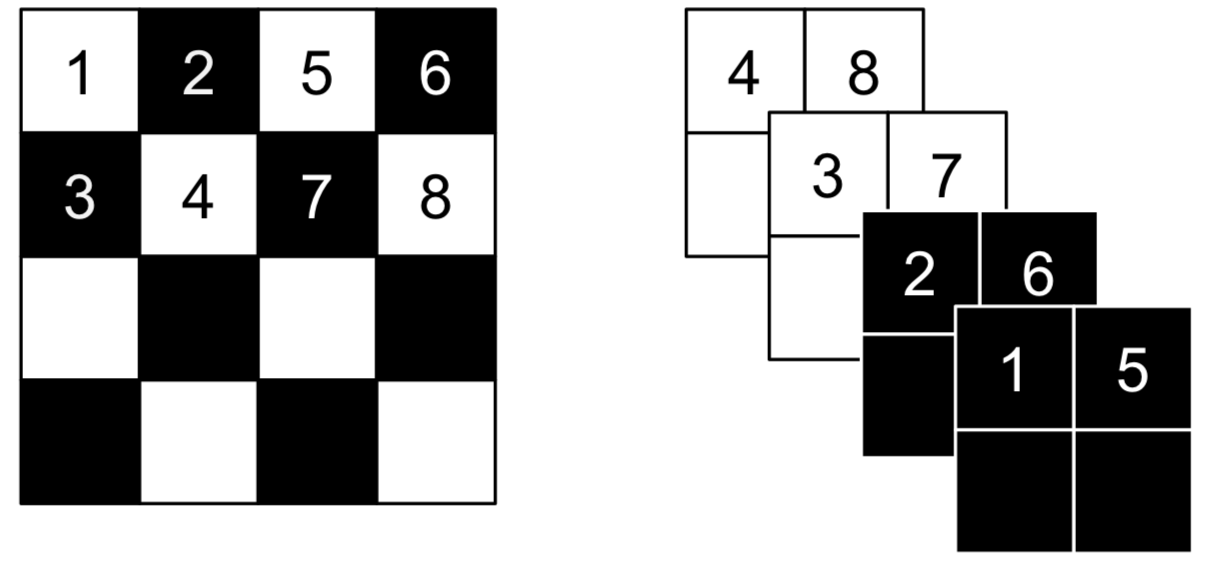
\includegraphics[width=0.75\linewidth]{figs/realnvp_masking.png}
	\end{figure}
	Masked convolutions are used to define ordering.
	
	\myfootnotewithlink{https://arxiv.org/abs/1605.08803}{Dinh L., Sohl-Dickstein J., Bengio S. Density estimation using Real NVP, 2016} 
\end{frame}
%=======
\begin{frame}{RealNVP}
	\begin{figure}
		\centering
		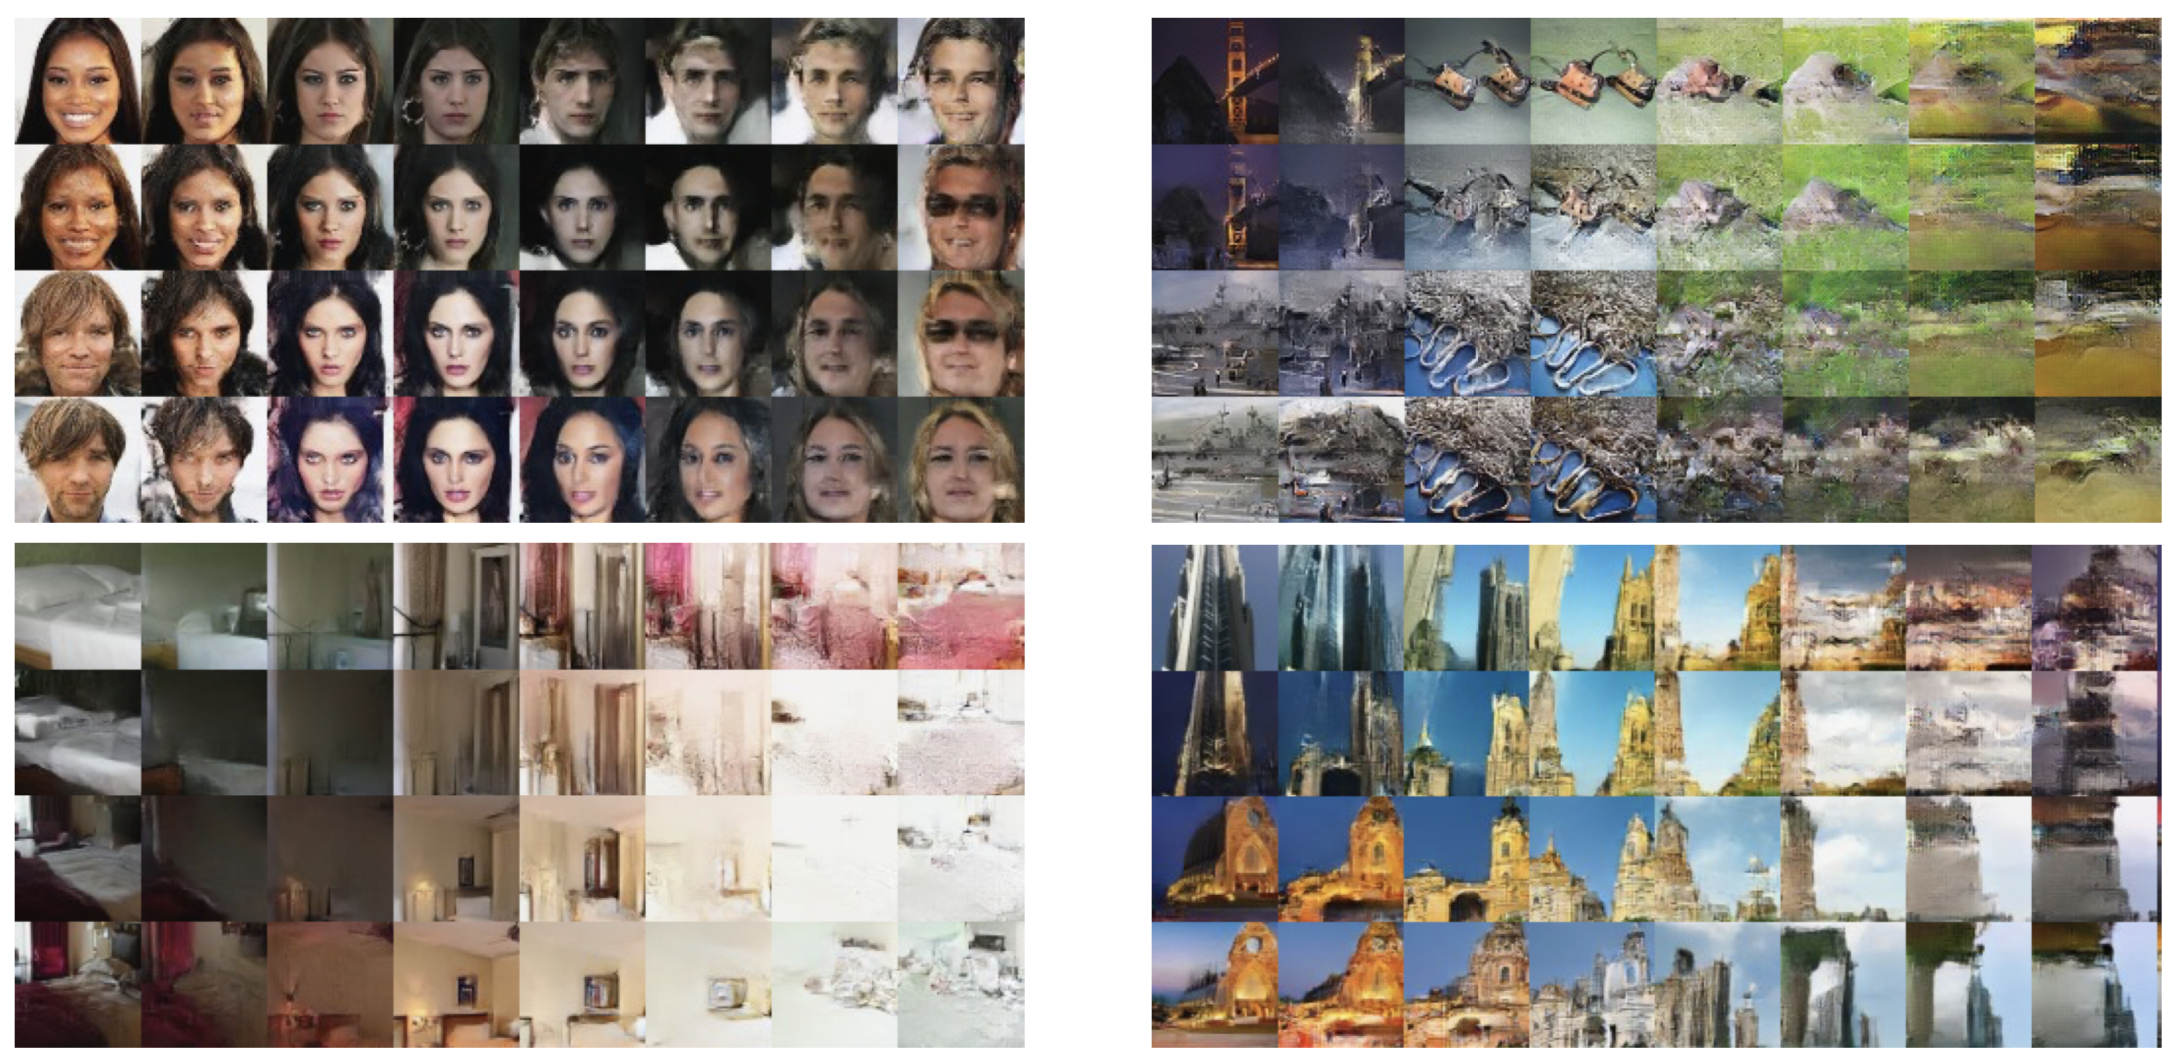
\includegraphics[width=\linewidth]{figs/realnvp_output.png}
	\end{figure}
	\myfootnotewithlink{https://arxiv.org/abs/1605.08803}{Dinh L., Sohl-Dickstein J., Bengio S. Density estimation using Real NVP, 2016} 
\end{frame}
%=======
\begin{frame}{RevNets, 2017}
	\begin{minipage}[t]{0.6\columnwidth}
		\begin{itemize}
			\item Modern neural networks are trained via backpropagation.
			\item Residual networks are state of the art in image classification.
			\item Backpropagation requires storing the network activations.
		\end{itemize}
	\end{minipage}%
	\begin{minipage}[t]{0.4\columnwidth}
		\begin{figure}
			\centering
			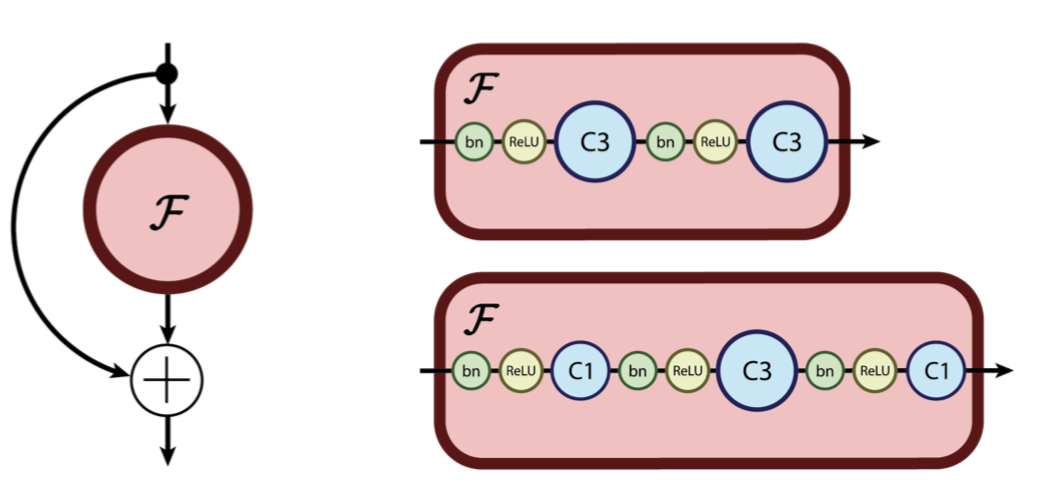
\includegraphics[width=\linewidth]{figs/resnet_block.png}
		\end{figure}
	\end{minipage}
	\vspace{0.1cm}
	\begin{block}{Problem}
		Storing the activations imposes an increasing memory burden. GPUs have limited memory capacity, leading to constraints often exceeded by state-of-the-art architectures (with thousand layers).
	\end{block}
	\myfootnotewithlink{https://arxiv.org/abs/1707.04585}{Gomez A. N. et al. The Reversible Residual Network: Backpropagation Without Storing Activations, 2017}
\end{frame}
%=======
\begin{frame}{RevNets, 2017}
	\begin{block}{NICE}
		\vspace{-0.2cm}
		\begin{equation*}
			\begin{cases} \bz_1 = \bx_1; \\ \bz_2 = \bx_2 + \mathcal{F}(\bx_1, \btheta);\end{cases}  \quad \Leftrightarrow \quad 
			\begin{cases} \bx_1 = \bz_1; \\ \bx_2 = \bz_2 - \mathcal{F}(\bz_1, \btheta).\end{cases} 
		\end{equation*}
		\vspace{-0.2cm}
	\end{block}
	\begin{block}{RevNet}
		\begin{equation*}
			\begin{cases} \by_1 = \bx_1 + \mathcal{F}(\bx_2, \btheta); \\ \by_2 = \bx_2 + \mathcal{G}(\by_1, \btheta);\end{cases} \quad \Leftrightarrow \quad 
			\begin{cases} \bx_2 = \by_2 - \mathcal{F}(\by_1, \btheta); \\ \bx_1 = \by_1 - \mathcal{G}(\bx_2, \btheta).\end{cases} 
		\end{equation*}
	\end{block}
	\begin{figure}
		\centering
		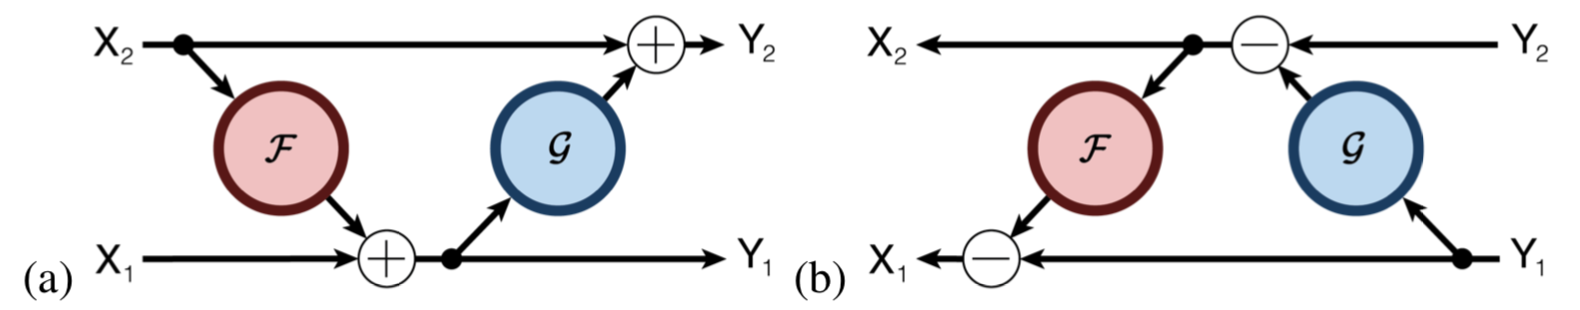
\includegraphics[width=\linewidth]{figs/revnet.png}
	\end{figure}
	\myfootnotewithlink{https://arxiv.org/abs/1707.04585}{Gomez A. N. et al. The Reversible Residual Network: Backpropagation Without Storing Activations, 2017}
\end{frame}
%=======
\begin{frame}{RevNets, 2017}
	\begin{figure}
		\centering
		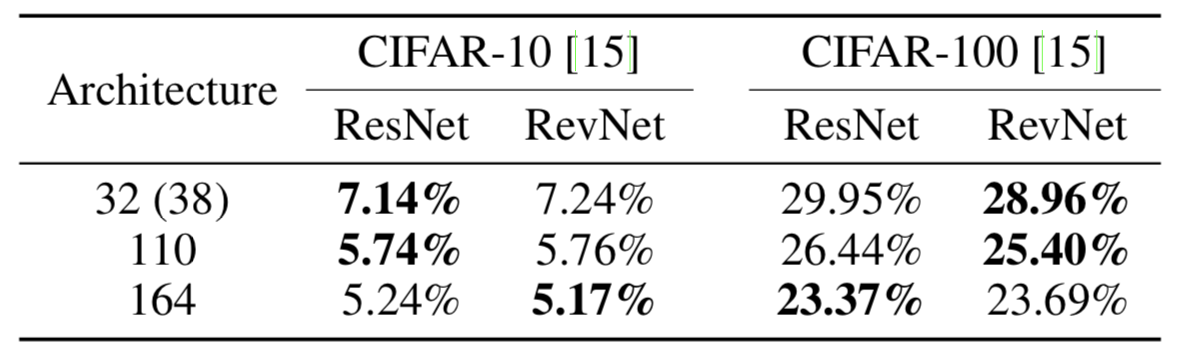
\includegraphics[width=0.8\linewidth]{figs/revnet_results.png}
	\end{figure}
	\begin{itemize}
		\item If the network contains non-reversible blocks (poolings, strides), activations for these blocks should be stored.
		\item To avoid storing activations in the modern frameworks, the backward pass should be manually redefined.
	\end{itemize}
	\myfootnotewithlink{https://arxiv.org/abs/1707.04585}{Gomez A. N. et al. The Reversible Residual Network: Backpropagation Without Storing Activations, 2017}
\end{frame}
%=======
\begin{frame}{i-RevNet, 2018}
	\begin{block}{Hypothesis}
		The success of deep convolutional networks is based on progressively discarding uninformative variability about the input with respect to the problem at hand. 
	\end{block}
	\begin{itemize}
		\item It is difficult to recover images from their hidden representations. 
		\item Information bottleneck principle: an optimal representation must reduce the MI between an input and its representation to reduce uninformative variability + maximize the MI between the output and its representation to preserve each class from collapsing onto other classes.
	\end{itemize}
	\myfootnotewithlink{https://arxiv.org/abs/1802.07088}{Jacobsen J. H., Smeulders A., Oyallon E. i-RevNet: Deep Invertible Networks, 2018}
\end{frame}
%=======
\begin{frame}{i-RevNet, 2018}
	\begin{block}{Hypothesis}
		The success of deep convolutional networks is based on progressively discarding uninformative variability about the input with respect to the problem at hand. 
	\end{block}
	
	\begin{block}{Idea}
		Build a cascade of homeomorphic layers (i-RevNet), a network that can be fully inverted up to the final projection onto the classes, i.e. no information is discarded.
	\end{block}
	\myfootnotewithlink{https://arxiv.org/abs/1802.07088}{Jacobsen J. H., Smeulders A., Oyallon E. i-RevNet: Deep Invertible Networks, 2018}
\end{frame}
%=======
\begin{frame}{i-RevNet, 2018}
	
	\begin{figure}
		\centering
		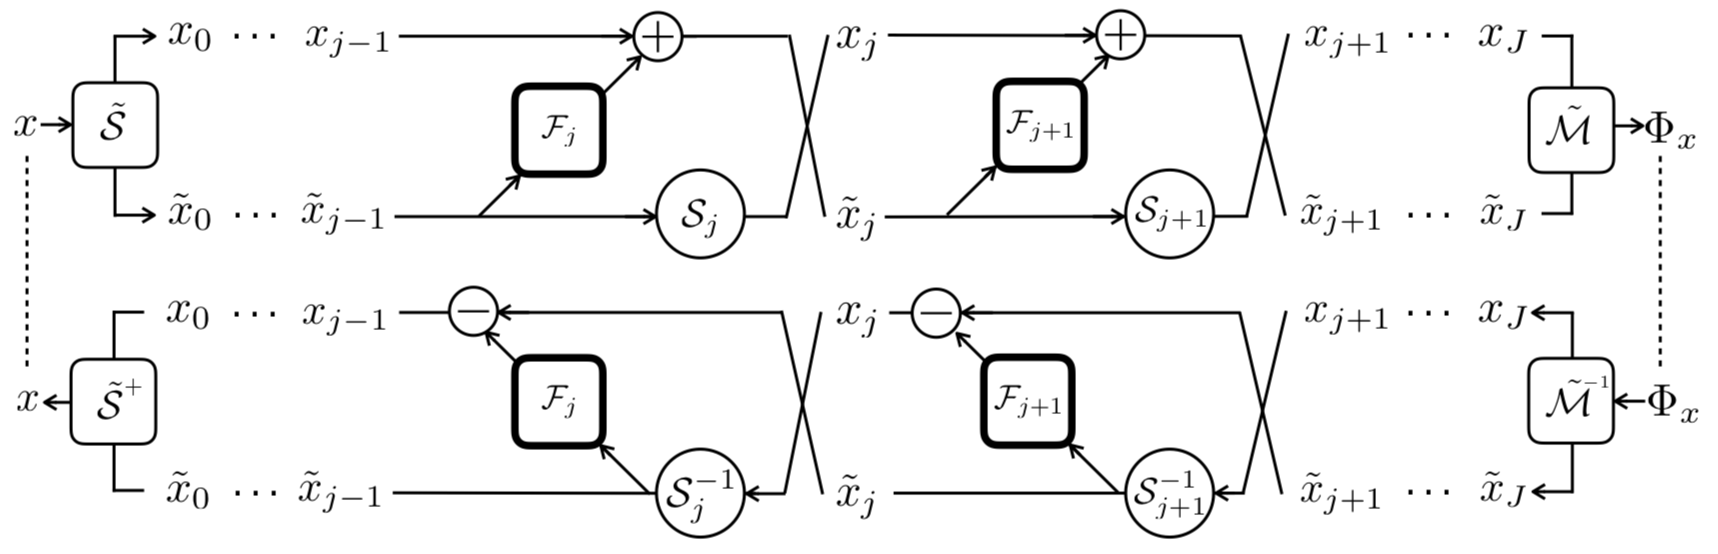
\includegraphics[width=\linewidth]{figs/i-revnet.png}
	\end{figure}
	
	\begin{figure}
		\centering
		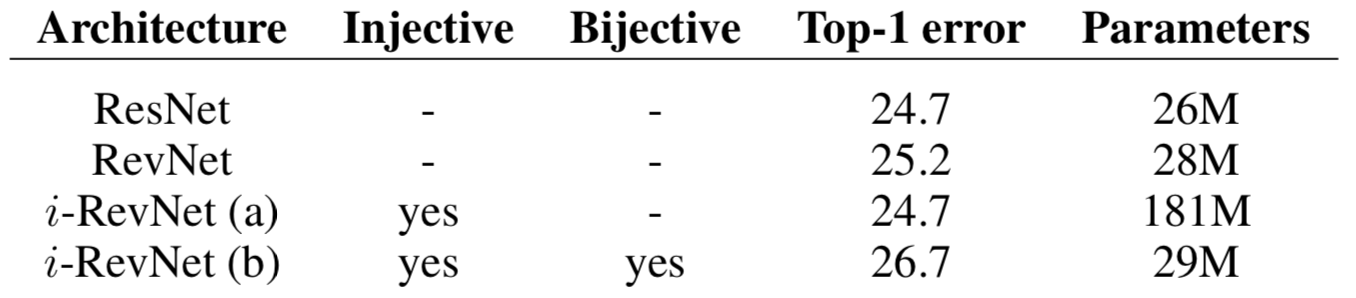
\includegraphics[width=0.9\linewidth]{figs/i-revnet_block.png}
	\end{figure}

	\myfootnotewithlink{https://arxiv.org/abs/1802.07088}{Jacobsen J. H., Smeulders A., Oyallon E. i-RevNet: Deep Invertible Networks, 2018}
\end{frame}
%=======
\begin{frame}{Summary}
\end{frame}
\end{document} 